% Figure 3.1. Local orthonormal frames on sub-simplices of a triangle and the
% normal/tangential symmetric tensor components (red: shared, black: element-private).
% Build in WSL: pdflatex for PDF, pdftocairo -eps for EPS, pdftocairo -png -r 300 for PNG.
\documentclass[tikz,border=3pt]{standalone}
\usepackage{amsmath}
\usepackage{tikz}
\usetikzlibrary{arrows.meta,calc}

\definecolor{shared}{RGB}{220,0,0}
\tikzset{
  frame/.style={line width=1.1pt,-{Latex[length=3mm,width=2mm]}},
  dof/.style={dashed,line width=0.6pt},
  lab/.style={circle,draw,inner sep=0.6pt,minimum size=4.2mm,font=\footnotesize}
}

% \frameDOF{P}{a}{b}{c1}{c2}{c3}
% P：标架原点；a、b：单位向量（b 为 a 顺时针旋转 90 度）；
% c1、c2、c3：分量 sym(a⊗a)、sym(a⊗b)、sym(b⊗b) 的标记颜色。
\newcommand{\frameDOF}[6]{
  \coordinate (P) at #1;
  \coordinate (A) at #2;
  \coordinate (B) at #3;
  \coordinate (Ta) at ($(P)+1.4*(A)$);
  \coordinate (Tb) at ($(P)+1.4*(B)$);
  \coordinate (D) at ($0.7071*(A)+0.7071*(B)$);
  \draw[frame] (P) -- (Ta);
  \draw[frame] (P) -- (Tb);
  % ① a⊗a
  \draw[dof,#4] ($(P)+1.15*(A)$) circle (0.36);
  \node[lab,#4] at ($(P)+1.15*(A)+0.62*(D)$) {1};
  % ② sym(a⊗b)
  \draw[dof,#5,{Stealth[length=1.6mm]}-{Stealth[length=1.6mm]}]
    ($(P)+0.62*(A)$) to[bend left=50] ($(P)+0.62*(B)$);
  \node[lab,#5] at ($(P)+1.2*(D)$) {2};
  % ③ b⊗b
  \draw[dof,#6] ($(P)+1.15*(B)$) circle (0.36);
  \node[lab,#6] at ($(P)+1.15*(B)+0.62*(D)$) {3};
}

\begin{document}
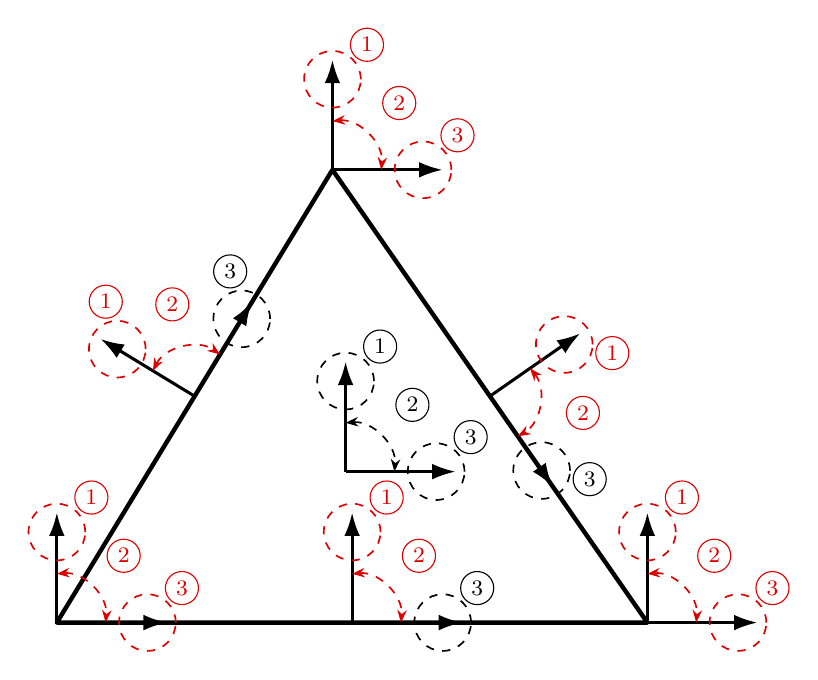
\begin{tikzpicture}[x=1cm,y=1cm]
  % 三角形顶点
  \coordinate (V1) at (0,0);
  \coordinate (V2) at (7.5,0);
  \coordinate (V3) at (3.5,5.75);

  \draw[line width=1.6pt,line join=round] (V1) -- (V2) -- (V3) -- cycle;

  % ================= 顶点：全局笛卡尔标架，三个分量均共享 =================
  \frameDOF{(V1)}{(0,1)}{(1,0)}{shared}{shared}{shared}
  \frameDOF{(V2)}{(0,1)}{(1,0)}{shared}{shared}{shared}
  \frameDOF{(V3)}{(0,1)}{(1,0)}{shared}{shared}{shared}

  % ================= 边：(n_e, t_e) 标架，n⊗n 与 sym(t⊗n) 共享，t⊗t 私有 =================
  % 底边：n_e 取向上（指向单元内部），t_e 自左向右
  \frameDOF{($(V1)!0.5!(V2)$)}{(0,1)}{(1,0)}{shared}{shared}{black}
  % 左边：t_e 自 V1 指向 V3，n_e 指向单元外部
  \frameDOF{($(V1)!0.5!(V3)$)}{(-0.8543,0.5199)}{(0.5199,0.8543)}{shared}{shared}{black}
  % 右边：t_e 自 V3 指向 V2，n_e 指向单元外部
  \frameDOF{($(V3)!0.5!(V2)$)}{(0.8209,0.5711)}{(0.5711,-0.8209)}{shared}{shared}{black}

  % ================= 单元内部：全局标架，三个分量均私有 =================
  \frameDOF{(3.667,1.917)}{(0,1)}{(1,0)}{black}{black}{black}
\end{tikzpicture}
\end{document}
